\documentclass[10pt]{beamer}
\usepackage[english]{babel}
\usepackage[utf8]{inputenc}
\usepackage[T1]{fontenc}
\usepackage{helvet}
\usepackage{listings}

%-------------------------------------------------------
% INFORMATION IN THE TITLE PAGE
%-------------------------------------------------------

\newcommand{\cstitle}{\textbf{Plataforma distribuída con Spark para el análisis de secuencias Next-generation}}
\subtitle[]{HPC}
\newcommand{\cscourseCode}{1005155}
\newcommand{\csauthor}{MSc. Vicente Machaca Arceda}
%\institute[UNSA]{Universidad Nacional de San Agustín de Arequipa}
\newcommand{\csemail}{vmachacaa@unsa.edu.pe}
\newcommand{\instituteabr}{UNSA}
\newcommand{\nameUp}{ICC Fase 1}
\date{\today}
\title[\cscourseCode]{\cstitle}
\author{\csauthor}
%%%%%%%%%%%%%%%%%

%-------------------------------------------------------
% CHOOSE THE THEME
%-------------------------------------------------------
\def\mycmd{0} % CS THEME
\def\mycmd{1} % MYTHEME
%-------------------------------------------------------

\if\mycmd1
	\usetheme[]{Feather}
	\newcommand{\chref}[2]{	\href{#1}{{\usebeamercolor[bg]{Feather}#2}} }
\else
	\usepackage{csformat}
\fi

\newcommand{\1}{
        	\setbeamertemplate{background}{
        		
\includegraphics[width=\paperwidth,height=\paperheight]{img/1}
        		\tikz[overlay] \fill[fill opacity=0.75,fill=white] (0,0) rectangle (-\paperwidth,\paperheight);
        	}
}



%-------------------------------------------------------
% THE BODY OF THE PRESENTATION
%-------------------------------------------------------

\begin{document}


\AtBeginSection[]
{
    \begin{frame}
        \frametitle{Table of Contents}
        \tableofcontents[currentsection]
    \end{frame}
}


%-------------------------------------------------------
% THE TITLEPAGE
%-------------------------------------------------------

\if\mycmd1 % MY THEME
	\1{
	\begin{frame}[plain,noframenumbering] 
		\titlepage 
	\end{frame}}

\else % CS THEME
	\maketitle
\fi


%-------------------------------------------------------
%-------------------------------------------------------
\begin{frame}{Overview}
	\tableofcontents
\end{frame}
%-------------------------------------------------------
%-------------------------------------------------------

%%%%%%%%%%%%%%%%%%%%%%%%%%%%%%%%%%%%%%%%%%%%%%%%%%%%%%%%
%%%%%%%%%%%%%%%%%%%%%%%%%%%%%%%%%%%%%%%%%%%%%%%%%%%%%%%%
\section{Introducción}
%%%%%%%%%%%%%%%%%%%%%%%%%%%%%%%%%%%%%%%%%%%%%%%%%%%%%%%%
%%%%%%%%%%%%%%%%%%%%%%%%%%%%%%%%%%%%%%%%%%%%%%%%%%%%%%%%

%%%%%%%%%%%%%%%%%%%%%%%%%%%%%%%%%%%%%%%%%%%%%%%%%%%%%%%%
\subsection{Problema}
%%%%%%%%%%%%%%%%%%%%%%%%%%%%%%%%%%%%%%%%%%%%%%%%%%%%%%%%

%-------------------------------------------------------
%-------------------------------------------------------
\begin{frame}{Problema}{}
	\begin{block}{}
		El análisis de secuencias de ADN obtenidas por \textit{Next-generation sequencing} es una tarea vital en los estudios de Bioinformática. Pero lamentablemente, las herramientas tradicionales no lentas y no aprovechan el poder computacional de un sistema distribuído
	\end{block}
\end{frame}
%-------------------------------------------------------
%-------------------------------------------------------

%%%%%%%%%%%%%%%%%%%%%%%%%%%%%%%%%%%%%%%%%%%%%%%%%%%%%%%%
\subsection{Objetivos}
%%%%%%%%%%%%%%%%%%%%%%%%%%%%%%%%%%%%%%%%%%%%%%%%%%%%%%%%

%-------------------------------------------------------
%-------------------------------------------------------
\begin{frame}{Objetivos}{}
	\begin{block}{}
		Desarrollar una herramienta para el análisis de secuencias obtenidas de \textit{Next-generation sequencing}. 
	\end{block}

	\begin{block}{}
		En esta versión, se implemento la funcionalidad para analizar la calidad de las lecturas.
	\end{block}
\end{frame}
%-------------------------------------------------------
%-------------------------------------------------------




%%%%%%%%%%%%%%%%%%%%%%%%%%%%%%%%%%%%%%%%%%%%%%%%%%%%%%%%
%%%%%%%%%%%%%%%%%%%%%%%%%%%%%%%%%%%%%%%%%%%%%%%%%%%%%%%%
\section{Marco teórico}
%%%%%%%%%%%%%%%%%%%%%%%%%%%%%%%%%%%%%%%%%%%%%%%%%%%%%%%%
%%%%%%%%%%%%%%%%%%%%%%%%%%%%%%%%%%%%%%%%%%%%%%%%%%%%%%%%

%-------------------------------------------------------
%-------------------------------------------------------
\begin{frame}{Secuenciamiento de ADN}{}
	\begin{figure}[H]
	\centering
	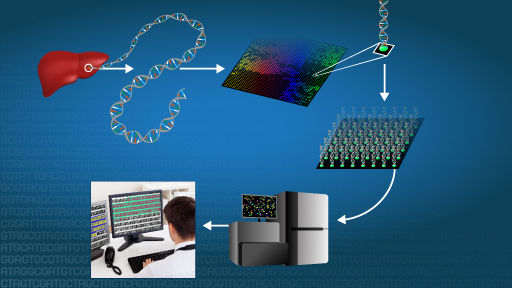
\includegraphics[width=0.8\textwidth]{img/proy/seq_1}
	\caption{Secuenciamiento de ADN}
\end{figure}
\end{frame}
%-------------------------------------------------------
%-------------------------------------------------------

%-------------------------------------------------------
%-------------------------------------------------------
\begin{frame}{Next-generation sequencing}{}
	\begin{figure}[H]
		\centering
		
\includegraphics[width=0.8\textwidth]{img/proy/seq_2}
		\caption{Next-generation sequencing}
	\end{figure}
\end{frame}
%-------------------------------------------------------
%-------------------------------------------------------

%-------------------------------------------------------
%-------------------------------------------------------
\begin{frame}{Single cell RNAseq}{}
	\begin{figure}[H]
		\centering
		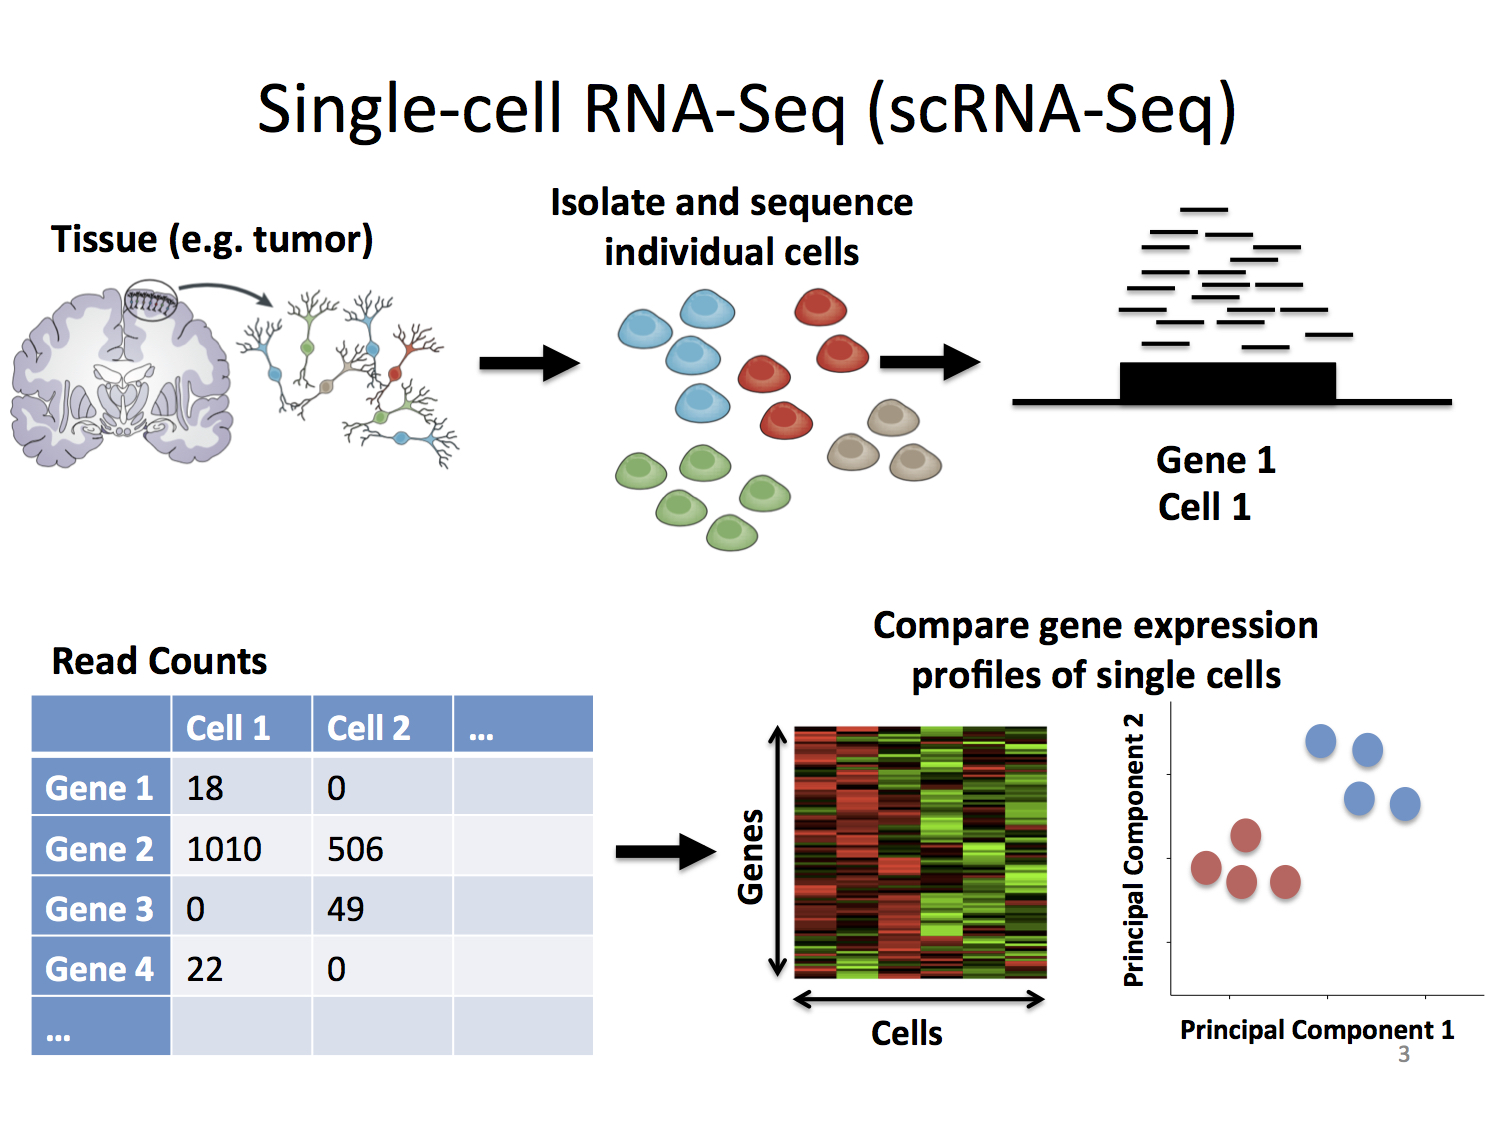
\includegraphics[width=0.8\textwidth]{img/proy/seq_3}
		\caption{Single cell RNAseq}
	\end{figure}
\end{frame}
%-------------------------------------------------------
%-------------------------------------------------------


%%%%%%%%%%%%%%%%%%%%%%%%%%%%%%%%%%%%%%%%%%%%%%%%%%%%%%%%
%%%%%%%%%%%%%%%%%%%%%%%%%%%%%%%%%%%%%%%%%%%%%%%%%%%%%%%%
\section{Propuesta}
%%%%%%%%%%%%%%%%%%%%%%%%%%%%%%%%%%%%%%%%%%%%%%%%%%%%%%%%
%%%%%%%%%%%%%%%%%%%%%%%%%%%%%%%%%%%%%%%%%%%%%%%%%%%%%%%%

%-------------------------------------------------------
%-------------------------------------------------------
\begin{frame}{Propuesta}{Análisis de secuencias}
	\begin{figure}[H]
		\centering
		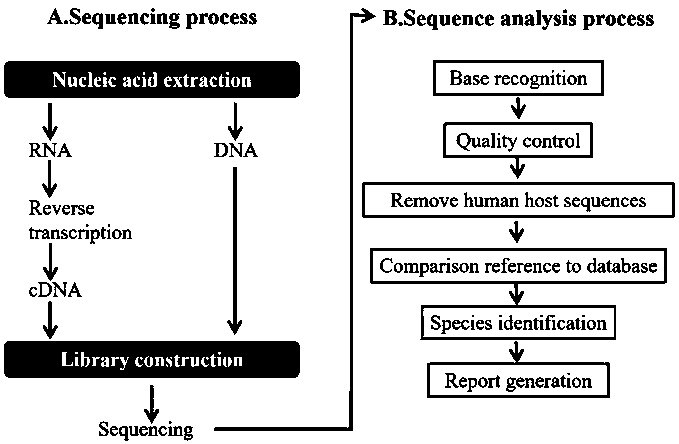
\includegraphics[width=0.8\textwidth]{img/proy/analysis2}
		\caption{Phases comunes realizadas en un análisis de secuencias de ADN (Next-generation).}
		\label{fig:analysis}
	\end{figure}	
\end{frame}
%-------------------------------------------------------
%-------------------------------------------------------

%-------------------------------------------------------
%-------------------------------------------------------
\begin{frame}{Propuesta}{Herramientas utilizadas}
\begin{table}[H]
	\centering
	\caption{Herramientas utilizadas para el proyecto}
	\label{tab:tools}
	\begin{tabular}{ll}
		\textbf{Herramienta} & \textbf{Version}
		\\ \hline
		Spark       & 3.2.0   \\
		Python      & 3.8.10  \\
		Pyspark     & 3.2.0  
	\end{tabular}
\end{table}	
\end{frame}
%-------------------------------------------------------
%-------------------------------------------------------

%-------------------------------------------------------
%-------------------------------------------------------
\begin{frame}{Propuesta}{Hardware}
\begin{table}[H]
	\centering
	\caption{Computadoras utilizadas en el sistema distribuído}
	\label{tab:pcs}
	\begin{tabular}{lp{6cm}}
		\textbf{Nombre de PC} & \textbf{Especificaciones}
		\\ \hline
		Desktop Asus      & Procesador i7 de séptima generación y 8GB de memoria RAM. Sistema operativo Linux.   \\
		Laptop Asus      & Procesador i5 de quinta generación y 4GB de memoria RAM. Sistema operativo Linux.\\
	\end{tabular}
\end{table}
\end{frame}
%-------------------------------------------------------
%-------------------------------------------------------

%-------------------------------------------------------
%-------------------------------------------------------
\begin{frame}{Propuesta}{Hardware}
	\begin{columns}
		\begin{column}{0.48\textwidth}
			\centering
			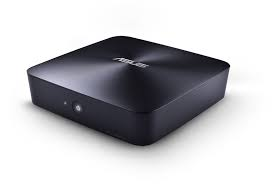
\includegraphics[width=\textwidth,height=0.5\textheight,keepaspectratio]{img/proy/pc_asus_1}
		\end{column}
	\begin{column}{0.48\textwidth}
		\centering
		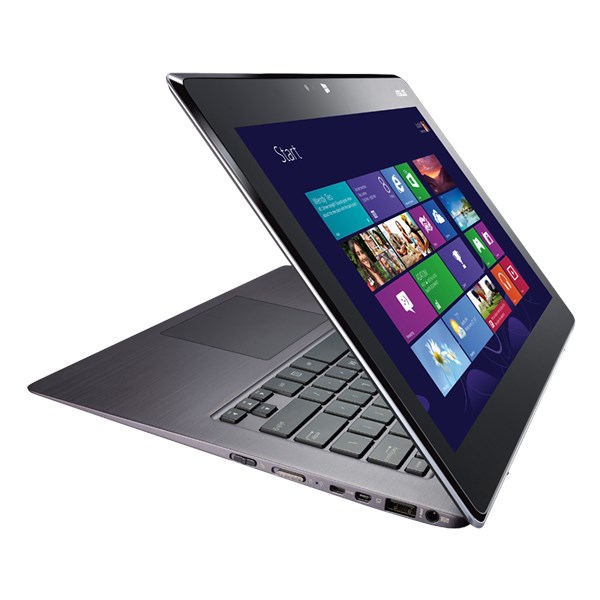
\includegraphics[width=\textwidth,height=0.5\textheight,keepaspectratio]{img/proy/pc_asus_2}
	\end{column}
	\end{columns}
\end{frame}
%-------------------------------------------------------
%-------------------------------------------------------

%-------------------------------------------------------
%-------------------------------------------------------
\begin{frame}{Propuesta}{Funcionalidades}
	\begin{itemize}
		\item Conteo de la cantidad de secuencias. 
		\item Conteo total de las bases nitrogenadas. 
		\item Computo de la longitud de todas las secuencias. 
		\item Computo del promedio de las longitudes de las secuenias.
		\item Computo de la ocurrencia de cada base nitrogenada.
		\item Análisis de contenido por base.
	\end{itemize}
\end{frame}
%-------------------------------------------------------
%-------------------------------------------------------


%%%%%%%%%%%%%%%%%%%%%%%%%%%%%%%%%%%%%%%%%%%%%%%%%%%%%%%%
%%%%%%%%%%%%%%%%%%%%%%%%%%%%%%%%%%%%%%%%%%%%%%%%%%%%%%%%
\section{Resultados}
%%%%%%%%%%%%%%%%%%%%%%%%%%%%%%%%%%%%%%%%%%%%%%%%%%%%%%%%
%%%%%%%%%%%%%%%%%%%%%%%%%%%%%%%%%%%%%%%%%%%%%%%%%%%%%%%%

%-------------------------------------------------------
%-------------------------------------------------------
\begin{frame}{Resultados}{}
\begin{block}{}
	Para evaluar el desempeño de la propuesta se evaluó las secuencias con el código \textbf{ERR3014700}, estas fueron descargadas de \href{https://www.ncbi.nlm.nih.gov/sra/ERR3014700}{NCBI}. 
\end{block}
\end{frame}
%-------------------------------------------------------
%-------------------------------------------------------

%-------------------------------------------------------
%-------------------------------------------------------
\begin{frame}[fragile]{Resultados}{Estadísticas}
\begin{figure}[]
	\centering
	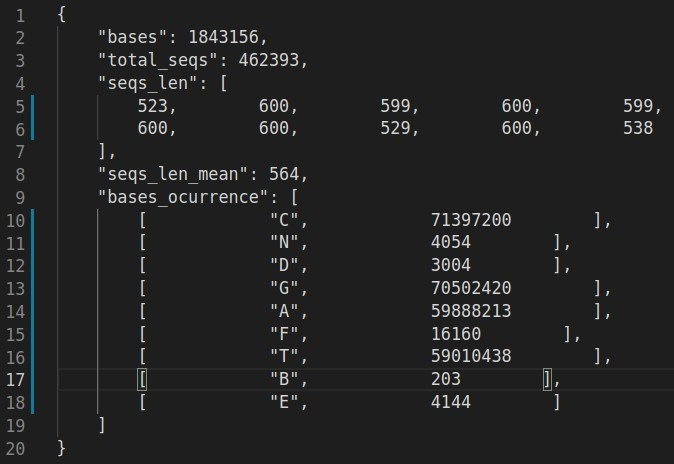
\includegraphics[width=\textwidth,height=0.7\textheight,keepaspectratio]{img/proy/json}
	%\label{img:mot2}
	\caption{Estadísticas de las lecturas.}
\end{figure}
\end{frame}
%-------------------------------------------------------
%-------------------------------------------------------

%-------------------------------------------------------
%-------------------------------------------------------
\begin{frame}{Resultados}{Análisis de contenido por base}
\begin{figure}[]
	\centering
	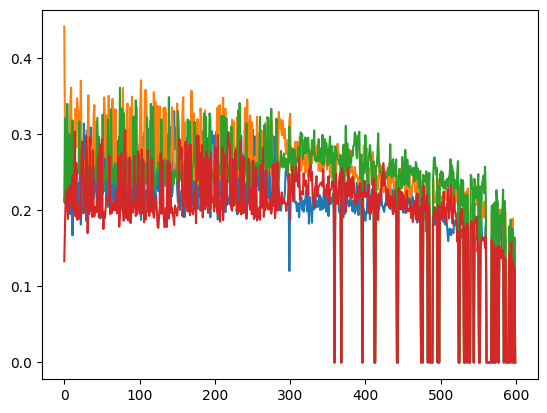
\includegraphics[width=\textwidth,height=0.7\textheight,keepaspectratio]{img/proy/per_base_content}
	%\label{img:mot2}
	\caption{Análisis de contenido por base.}
\end{figure}
\end{frame}
%-------------------------------------------------------
%-------------------------------------------------------


%%%%%%%%%%%%%%%%%%%%%%%%%%%%%%%%%%%%%%%%%%%%%%%%%%%%%%%%
%%%%%%%%%%%%%%%%%%%%%%%%%%%%%%%%%%%%%%%%%%%%%%%%%%%%%%%%
\section{Conclusiones}
%%%%%%%%%%%%%%%%%%%%%%%%%%%%%%%%%%%%%%%%%%%%%%%%%%%%%%%%
%%%%%%%%%%%%%%%%%%%%%%%%%%%%%%%%%%%%%%%%%%%%%%%%%%%%%%%%

%-------------------------------------------------------
%-------------------------------------------------------
\begin{frame}{Conclusiones}{}
	\begin{itemize}
		\item En este proyecto se ha desarrollado una herramienta distribuída que permite hacer el análisis masivo de grandes cantidades de lecturas de ADN (Next-generation sequencing). 
		
		\item El proyecto se enfoco en el análisis de calidad de las lecturas de ADN, este es un paso crucial en cualquier experimento de Bioinformática. Como resultado, la propuesta obtiene estadísticas referentes a las ocurrencias de las bases nitrogenadas y además se desarrollo un análisis de contenido por base. \\
	\end{itemize}
\end{frame}
%-------------------------------------------------------
%-------------------------------------------------------

%-------------------------------------------------------
%-------------------------------------------------------
\begin{frame}[allowframebreaks]
	\frametitle{References}
	%\bibliographystyle{amsalpha}
	\bibliographystyle{IEEEtran}
	\bibliography{bibliography}
\end{frame}
%-------------------------------------------------------
%-------------------------------------------------------


%-------------------------------------------------------
%-------------------------------------------------------
\if\mycmd1 % MY THEME
\1{
	{\1
		\begin{frame}[plain,noframenumbering]
			%\finalpage{Thank you}
			\begin{figure}[]
				\centering
				
\includegraphics[width=\textwidth,height=0.7\textheight,keepaspectratio]{img/question.png}
				%\label{img:mot2}
				%\caption{Image example in 2 gray levels.}
			\end{figure}
		\end{frame}}
	\else % CS THEME
		\begin{frame}{Questions?}
			\begin{figure}[]
				\centering
				
\includegraphics[width=\textwidth,height=0.7\textheight,keepaspectratio]{img/question.png}
				%\label{img:mot2}
				%\caption{Image example in 2 gray levels.}
			\end{figure}
			
		\end{frame}
\fi
%-------------------------------------------------------
%-------------------------------------------------------

\end{document}